% =============================
% ภาคผนวก
% =============================
% ใช้คำสั่ง \appendiceschapter{ชื่อภาคผนวก} สำหรับแต่ละภาคผนวก
% ระบบกำหนดตัวอักษร ก, ข, ค ... ให้เอง

% =============================
% ภาคผนวก ก
% =============================
\setcounter{chapter}{-1}
\appendiceschapter{หน้าจอสาธิตระบบ}

\section*{ภาพรวมของหน้าจอสาธิต}

โครงงานนี้พัฒนาหน้าจอสาธิตขึ้นเพื่อให้ทดลองใช้ระบบได้จริง และเพื่อให้เห็นความต่าง
ระหว่างสถาปัตยกรรมทั้งสามแบบขณะทำงาน หน้าจอนี้ทำงานบนเครื่องส่วนบุคคลเช่นเดียวกับ
ตัวระบบ และเรียกใช้สถาปัตยกรรมตัวจริงชุดเดียวกับที่ใช้วัดผลในบทที่ 4
ไม่ได้แสดงผลลัพธ์ที่เตรียมไว้ล่วงหน้า

หน้าจอหลักก่อนเริ่มถามคำถามแสดงดังภาพที่ \ref{fig:demo_ui}

\begin{figure}[H]
\centering
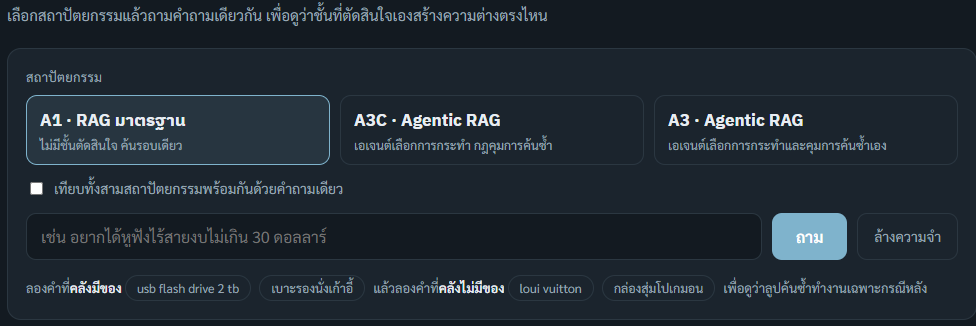
\includegraphics[width=\textwidth]{images/demo-ui.png}
\caption{หน้าจอหลักของระบบสาธิต ส่วนเลือกสถาปัตยกรรมและช่องพิมพ์คำถาม}
\label{fig:demo_ui}
\end{figure}

ส่วนประกอบของหน้าจอแบ่งเป็น 4 ส่วน ดังนี้

\begin{enumerate}[label=\arabic*)]
    \item \textbf{ส่วนเลือกสถาปัตยกรรม} ผู้ใช้เลือกได้ว่าจะให้คำถามนี้ทำงานด้วย A1 ซึ่งเป็น
          RAG มาตรฐาน A3C ซึ่งเป็น Agentic RAG ที่เอเจนต์เลือกการกระทำ หรือ A3
          ซึ่งเอเจนต์คุมการค้นซ้ำเองด้วย ใต้ชื่อแต่ละแบบมีคำอธิบายสั้นกำกับว่าต่างกันอย่างไร
    \item \textbf{ตัวเลือกเทียบทั้งสามแบบพร้อมกัน} เมื่อเปิดใช้ ระบบจะส่งคำถามเดียวกัน
          ไปยังทั้งสามสถาปัตยกรรมแล้วแสดงผลเรียงลงมา ทำให้เปรียบเทียบได้ในคราวเดียว
    \item \textbf{ช่องพิมพ์คำถาม} รับได้ทั้งภาษาไทยและภาษาอังกฤษ ระบบตรวจภาษาเองแล้วตอบ
          เป็นภาษาเดียวกับที่ถาม ข้างล่างมีคำค้นตัวอย่างที่กดใช้ได้ทันที
          แบ่งเป็นกลุ่มที่คลังมีสินค้าและกลุ่มที่คลังไม่มีสินค้า
    \item \textbf{ปุ่มล้างความจำ} เนื่องจากแต่ละสถาปัตยกรรมจดจำบทสนทนาข้ามรอบ
          การเริ่มคำถามใหม่ที่ไม่เกี่ยวกับคำถามก่อนจึงต้องล้างความจำก่อน
\end{enumerate}

\section*{ผลการเปรียบเทียบสามสถาปัตยกรรมด้วยคำถามเดียวกัน}

ภาพที่ \ref{fig:demo_compare} แสดงผลเมื่อเปิดโหมดเทียบทั้งสามแบบ แล้วถามด้วยคำค้น
\texttt{loui vuitton} ซึ่งเป็นคำค้นจริงจากชุดทดสอบในกลุ่มที่คลังไม่มีสินค้าตรง
และเป็นคำที่ผู้ใช้สะกดผิดจากคำว่า louis vuitton

\begin{figure}[H]
\centering
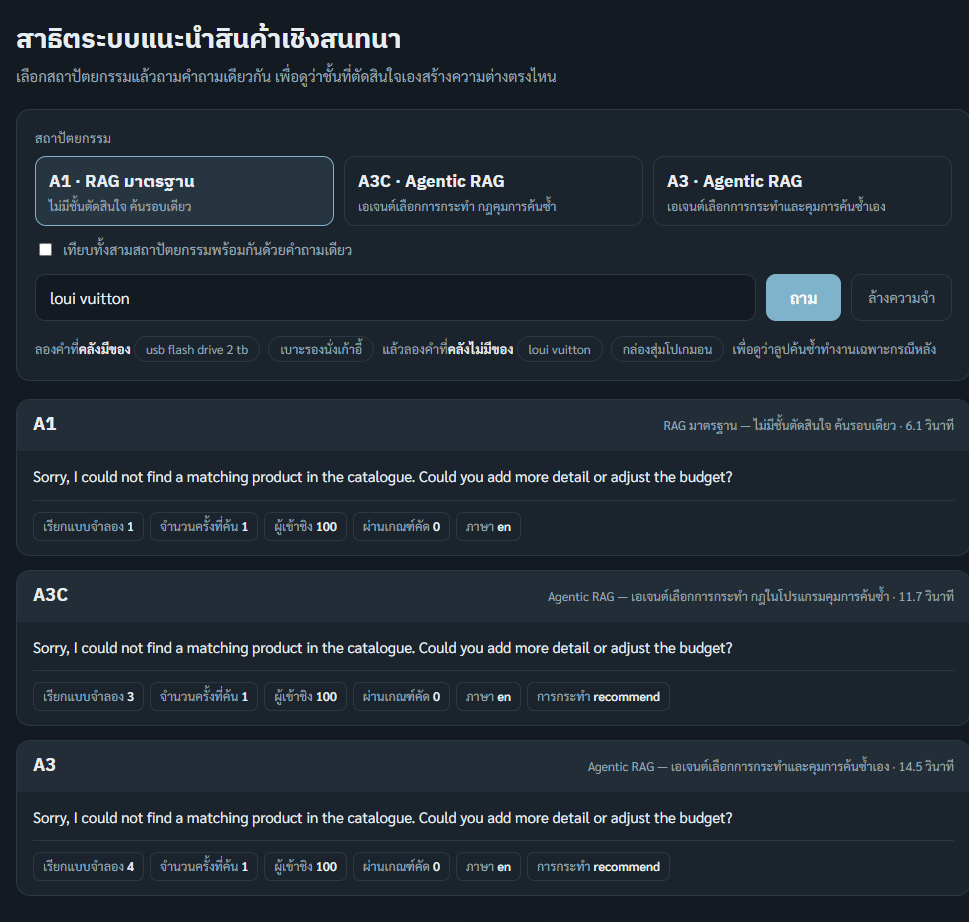
\includegraphics[width=\textwidth]{images/demo-compare.png}
\caption{ผลการเปรียบเทียบทั้งสามสถาปัตยกรรมด้วยคำถามเดียวกัน}
\label{fig:demo_compare}
\end{figure}

\subsection*{การอ่านผลในภาพ}

ใต้คำตอบของแต่ละสถาปัตยกรรมมีแถบตัวเลขที่ดึงมาจากการทำงานจริงของรอบนั้น
ได้แก่ จำนวนครั้งที่เรียกแบบจำลองภาษา จำนวนครั้งที่ค้น จำนวนผู้เข้าชิงที่ดึงมาจากคลัง
จำนวนที่ผ่านเกณฑ์คัด ภาษาที่ตรวจได้ และการกระทำที่ชั้นวางแผนเลือก
สรุปค่าที่ปรากฏในภาพได้ดังตารางที่ \ref{tab:demo_trace}

\begin{table}[H]
\centering
\caption{ค่าที่วัดได้จากหน้าจอสาธิตในภาพที่ \ref{fig:demo_compare}}
\label{tab:demo_trace}
\begin{tabular}{|l|c|c|c|}
\hline
\textbf{รายการ} & \textbf{A1} & \textbf{A3C} & \textbf{A3} \\
\hline
เรียกแบบจำลองภาษา (ครั้ง) & \textbf{1} & 3 & 4 \\ \hline
จำนวนครั้งที่ค้น & 1 & 1 & 1 \\ \hline
ผู้เข้าชิงที่ดึงจากคลัง & 100 & 100 & 100 \\ \hline
ผ่านเกณฑ์คัด & 0 & 0 & 0 \\ \hline
เวลาที่ใช้ (วินาที) & \textbf{6.1} & 11.7 & 14.5 \\ \hline
คำตอบ & ไม่พบ & ไม่พบ & ไม่พบ \\
\hline
\end{tabular}
\end{table}

สิ่งที่ภาพนี้แสดงมี 3 ประการ

\begin{enumerate}[label=\arabic*)]
    \item \textbf{ทั้งสามสถาปัตยกรรมปฏิเสธถูกต้องตรงกัน} เนื่องจากไม่มีสินค้าใด
          ผ่านเกณฑ์คัดเลยแม้แต่ชิ้นเดียว ระบบจึงตอบว่าไม่พบแทนที่จะเสนอสินค้าที่ไม่ตรง
          ซึ่งเป็นพฤติกรรมที่ถูกต้องสำหรับคำค้นกลุ่มนี้
    \item \textbf{ต้นทุนเพิ่มขึ้นตามความเป็นเอเจนต์ แต่ผลลัพธ์เท่ากัน} A1 เรียกแบบจำลอง
          เพียงครั้งเดียวและใช้เวลา 6.1 วินาที ขณะที่ A3 เรียก 4 ครั้งและใช้เวลา 14.5 วินาที
          หรือราว 2.4 เท่า ทั้งที่ได้คำตอบเหมือนกันทุกประการ
          ข้อสังเกตนี้สอดคล้องกับข้อสรุปในบทที่ 5 ที่ว่าการขยายขอบเขตการตัดสินใจของ
          เอเจนต์ไปถึงการคุมการค้นซ้ำนั้นไม่คุ้มกับต้นทุนที่เพิ่มขึ้น
    \item \textbf{ชั้นวางแผนทำงานจริง} A3C และ A3 แสดงการกระทำที่เลือกไว้ว่า recommend
          ขณะที่ A1 ไม่มีช่องนี้เพราะไม่มีชั้นวางแผน จึงค้นทันทีทุกครั้ง
\end{enumerate}

\subsection*{ข้อสังเกตเรื่องความจำกับการสาธิต}

ในภาพที่ \ref{fig:demo_compare} จำนวนครั้งที่ค้นของทั้งสามสถาปัตยกรรมเท่ากับ 1
กล่าวคือ\textbf{การค้นซ้ำไม่ได้ทำงาน} ทั้งที่คำค้นนี้อยู่ในกลุ่มที่คลังไม่มีสินค้า
สาเหตุคือรอบนั้นได้ถามคำถามเดียวกันไปก่อนหน้าแล้ว ระบบจึงจดจำไว้ว่าเคยพยายามค้นด้วย
คำนี้แล้วไม่พบ และไม่พยายามซ้ำอีก

เมื่อล้างความจำแล้วถามใหม่ด้วยคำเดียวกัน การค้นซ้ำทำงานตามที่ออกแบบไว้ คือค้น 2 รอบ
และเรียกแบบจำลองภาษา 4 ครั้งสำหรับ A3C โดยคำค้นที่ระบบเขียนขึ้นใหม่ในรอบที่สองคือ
louis vuitton ซึ่งเป็นการแก้คำสะกดจาก loui vuitton ได้ถูกต้อง
กรณีนี้สำเร็จเพราะเป็นชื่อแบรนด์ที่แบบจำลองรู้จัก ไม่ใช่ความสามารถแก้คำสะกดทั่วไป
ตามที่อธิบายไว้ในบทที่ 4

ข้อสังเกตนี้มีผลเชิงปฏิบัติคือ \textbf{การสาธิตควรล้างความจำก่อนเริ่มคำถามใหม่ทุกครั้ง}
มิฉะนั้นพฤติกรรมการค้นซ้ำจะไม่ปรากฏให้เห็น

\section*{วิธีเรียกใช้งาน}

ระบบสาธิตต้องเปิดบริการแบบจำลองภาษาในเครื่องก่อน แล้วจึงเปิดเซิร์ฟเวอร์ของหน้าจอสาธิต
จากนั้นเข้าใช้งานผ่านเว็บเบราว์เซอร์ที่ที่อยู่ภายในเครื่อง
เซิร์ฟเวอร์เขียนด้วยไลบรารีมาตรฐานของภาษาไพทอนทั้งหมด จึงไม่ต้องติดตั้งเว็บเฟรมเวิร์กเพิ่ม
